\documentclass[11pt,nocut]{article}

\usepackage{../latex_style/packages}
\usepackage{../latex_style/notations}
%\externaldocument{../lecture_02/lecture_02}
\externaldocument{../lecture_07/lecture_07}


\title{\vspace{-2.0cm}%
	Optimization and Computational Linear Algebra for Data Science\\
Lecture 12: Gradient descent}
\author{Léo \textsc{Miolane} \ $\cdot$ \ \texttt{leo.miolane@gmail.com}}
\date{\today}

\begin{document}
\maketitle
\textbf{Warning:}
\emph{This material is not meant to be lecture notes. It only gathers the main concepts and results from the lecture, without any additional explanation, motivation, examples, figures...
}


\begin{center}
In these notes, $f$ denotes a twice differentiable \textbf{convex} function from $\R^n$ to $\R$.
\end{center}

\section{Gradient descent}

Given an initial point $x_0 \in \R^n$, the gradient descent algorithm follows the updates:
\begin{equation}\label{eq:gradient_step}
x_{t+1} = x_t - \alpha_t \nabla f(x_t),
\end{equation}
where the step-size $\alpha_t$ remains to be determined.
The step \eqref{eq:gradient_step} is a very natural strategy to minimize $f$, since $-\nabla f(x)$ is the direction of steepest descent at $x$. Since $f(x+h) = f(x) + \langle \nabla f(x), h \rangle + o(\|h\|)$ we have
\begin{align*}
f(x_{t+1}) 
&= f(x_t) - \alpha_t \| \nabla f(x_t) \|^2 + o(\alpha_t) \\
&< f(x_t) 
\end{align*}
for $\alpha_t$ small enough (provided that $\nabla f(x_t) \neq 0$).
Hence is the step-sizes $\alpha_t$ are chosen very small, the sequence $(f(x_t))_{t \geq 0}$ is decreasing!
However, if $\alpha_t$ are too small, the algorithm may never converge.

\subsection{Convergence analysis}


\textbf{Notation}: Given a symmetric matrix $M$ we will denote by $\lambda_{\rm min}(M)$ and $\lambda_{\rm max}(M)$ the smallest and largest eigenvalues of $M$. 
\begin{definition}\label{def:strong}
	For $L,\mu >0$, we say that a twice-differentiable convex function $f: \R^n \to \R$ is
	\begin{itemize}
		\item $L$-smooth if for all $x \in \R^n$, $\lambda_{\rm max}(H_f(x)) \leq L$.
		\item $\mu$-strongly convex if for all $x \in \R^n$, $\lambda_{\rm min}(H_f(x)) \geq \mu$.
	\end{itemize}
\end{definition}
\begin{remark}
	Smoothness and strong convexity are usually defined as follows. We say that $f$ is
	\begin{itemize}
		\item $L$-smooth if $f$ is differentiable and if its gradient is $L$-Lipschitz meaning that for all $x,y \in \R^n$, $\| \nabla f(x) - \nabla f(y) \| \leq L \|x-y\|$.
		\item $\mu$-strongly convex if the function $x \mapsto f(x) - \frac{\mu}{2} \|x\|^2$ is convex.
	\end{itemize}
	These definitions are more general since they do not require $f$ to be twice differentiable (for smoothness) or differentiable (for strong convexity). However, one can check that they are equivalent to Definition~\ref{def:strong} when $f$ is twice differentiable. In these notes, we will prefer to use Definition~\ref{def:strong} because it makes clear that these two assumptions are related to the eigenvalues of the Hessian of $f$.
\end{remark}

\begin{remark}\label{rem:sandwich}
	$L$-smooth and $\mu$-strongly convex functions are very convenient since they can be ``sandwiched'' as follows (see homework 9 for a proof):
	$$
	f(x) + \langle h ,\nabla f(x) \rangle + \frac{\mu}{2} \|h\|^2 
	\leq f(x+h) \leq
	f(x) + \langle h ,\nabla f(x) \rangle + \frac{L}{2} \|h\|^2,
	$$
	for all $x,h \in\R^n$.
\end{remark}

\begin{theorem}\label{th:gradient1}
	Assume that $f$ is $L$-smooth and that $f$ admits a (global) minimizer $x^* \in \R^n$. Then
	the gradient descent iterates \eqref{eq:gradient_step} with constant step-size $\alpha_k = 1/L$ verify
	$$
	f(x_t) - f(x^*) \leq \frac{2 L \| x_0 - x^* \|^2}{t+4}.
	$$
\end{theorem}
See Section 2.1.5 from \cite{nesterov2018lectures} for a proof.

\paragraph{Why did we used step sizes of $1/L$ ?} $f$ is $L$-smooth, hence (see Remark \ref{rem:sandwich}) for all $x,h \in \R^n$:
\begin{equation}\label{eq:upperL}
f(x+h) \leq f(x) + \langle \nabla f(x) , h \rangle + \frac{L}{2} \|h\|^2.
\end{equation}
Then, one can check (exercise!) that when $x$ is fixed, the minimum of the right-hand side is minimum for $h = - \frac{1}{L} \nabla f(x)$.

\begin{theorem}\label{th:gradient2}
	Assume that $f$ is $L$-smooth and $\mu$-strongly convex. 
	Then $f$ admits a unique minimizer global $x^*$ and
	the gradient descent iterates \eqref{eq:gradient_step} with constant step-size $\alpha_k = 1/L$ verify
	$$
	f(x_t) - f(x^*) \leq \Big(1-\frac{\mu}{L}\Big)^t (f(x_0) - f(x^*)).
	$$
\end{theorem}
\begin{remark}
	Theorems~\ref{th:gradient1}-\ref{th:gradient2} show that gradient descent is adaptive to strong convexity of $f$.
\end{remark}
\begin{remark}
	The ratio $\kappa = \frac{L}{\mu} \geq 1$ is called the condition number. The smaller the condition number, the faster the convergence.
\end{remark}
%\begin{remark}
	%The $\mu$-strong convexity of $f$ implies (using Remark \ref{rem:sandwich}) that for all $x \in \R^n$,
	%$$
	%\frac{\mu}{2} \|x - x^* \|^2 \leq f(x)-f(x^*).
	%$$
	%Combining this with Theorem \ref{th:gradient2} gives a bound of the distance to the minimizer $x^*$:
	%$$
	%\|x_t - x^* \|^2 \leq \frac{2}{\mu}\Big(1-\frac{\mu}{L}\Big)^{\! t} (f(x_0) - f(x^*)).
	%$$
%\end{remark}

\begin{proof}
	Let $t \geq 0$. Applying \eqref{eq:upperL} for $x=x_t$ and $h=x_t - L^{-1} \nabla f(x_t)$, we get
	$$
	f(x_{t+1}) 
	\leq f(x_t) - \frac{1}{L} \|\nabla f(x_t) \|^2 + \frac{1}{2L}\|\nabla f(x_t) \|^2
	= f(x_t) - \frac{1}{2L} \|\nabla f(x_t) \|^2.
	$$
	Now, since $f$ is $\mu$-strongly convex, we have (exercise!) for all $x \in \R^n$
	\begin{equation}\label{eq:boundG}
f(x) - f(x^*) \leq 2 \mu \|\nabla f(x)\|^2.
	\end{equation}
We get that $f(x_{t+1}) \leq f(x_t) - \frac{\mu}{L}(f(x_t) - f(x^*))$, hence
$$
f(x_{t+1}) - f(x^*) \leq \Big(1 - \frac{\mu}{L}\Big)(f(x_t) - f(x^*)),
$$
from which the theorem follows.
\end{proof}

\subsection{Choosing the step size in practice}

In practice, one may not have access to $L$ and need hence to choose the step size $\alpha_t$. A popular method is the so-called ``backtracking line search'' a goes as follows.
Fix a parameter $\beta \in (0,1)$.
Start with $\alpha = 1$ and while
$$
f\big(x_t - \alpha \nabla f (x_t) \big) > f(x_t) - \frac{\alpha}{2} \|\nabla f(x_t) \|^2,
$$
update $\alpha =\beta \alpha$. Then choose $\alpha_t = \alpha$.

\subsection{Accelerated gradient method}

\begin{figure}[H]
	\begin{center}
		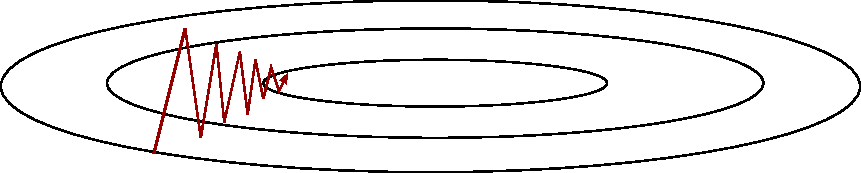
\includegraphics[width=0.47\textwidth]{figures/gd.pdf}
		\hspace{7mm}
		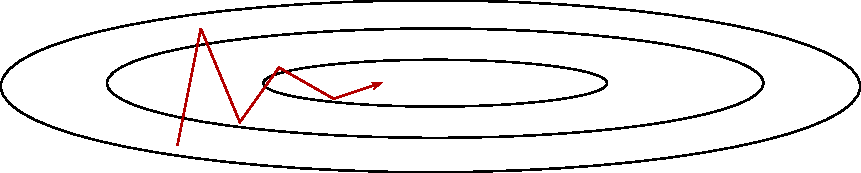
\includegraphics[width=0.47\textwidth]{figures/momentum.pdf}
		\caption{\emph{Left}: gradient descent may oscillate in narrow valleys. \emph{Right}: gradient descent with momentum accumulate momentum in the horizontal direction, while damping the oscillations on the vertical axis.}
	\end{center}
\end{figure}
\paragraph{Gradient descent with momentum.}

Also known as ``heavy ball'' method, this scheme was introduced by Polyak in 1964.
This is a way to prevent zigzagging trajectories when doing gradient descent by adding a momentum term:
\begin{align*}
	x_{t+1} = x_t + v_t
	\quad \text{where} \quad
	v_t = \alpha_t v_{t-1} - \beta_t \nabla f(x_{t}),
\end{align*}
for some $\alpha_t,\beta_t$. The idea is to keep momentum from past iterations in order to avoid zigzagging. It is possible to show that adding the momentum term leads to a better rate when $f$ is twice differentiable, $L$-smooth and $\mu$-strongly convex:
$$
\|x_t - x^*\| \leq \left(\frac{\sqrt{L}-\sqrt{\mu}}{\sqrt{L} + \sqrt{\mu}}\right)^{\! t} \|x_0 - x^*\|,
$$
when $\alpha_t$ and $\beta_t$ are appropriately chosen.


\paragraph{Nesterov's accelerated gradient descent.}

Nesterov's accelerated gradient descent uses the idea of momentum, but evaluate the gradient at a different point that $x_t$:
\begin{align*}
	x_{t+1} = x_t + v_t
	\quad \text{where} \quad
	v_t = \alpha_t v_{t-1} - \beta_t \nabla f(x_{t} + \alpha_t v_{t-1})
\end{align*}

When $\alpha_t,\beta_t$ are properly chosen, it improves on the convergence rates of gradient descent (given by Theorems~\ref{th:gradient1}-\ref{th:gradient2}). Namely:
\begin{itemize}
	\item if $f$ is $L$-smooth and if its minimum is attained at some $x^*$, then for $\alpha_t = \frac{t-1}{t+2}$ and $\beta_t = 1/L$ we have
		$$
		f(x_t) - f(x^*) \leq \frac{2L \|x_0-x^*\|^2}{(t+1)^2}.
		$$
	\item if $f$ is $L$-smooth and $\mu$-strongly convex, then for $\alpha_t = \frac{1-\sqrt{\mu/L}}{1+\sqrt{\mu/L}}$ and $\beta_t = 1/L$ we have
		$$
		f(x_t) - f(x^*) \leq L \|x_0-x^*\|^2 \Big(1-\sqrt{\mu/L}\Big)^t.
		$$
\end{itemize}
See for instance \cite{schmidt2011convergence} for proofs of these results.


\section{Newton's method}

\subsection{Newton's method}
We assume here that $f$ is $\mu$-strongly convex and $L$-smooth.
Newton's method performs updates according to
\begin{equation}\label{eq:newton}
	x_{t+1} = x_t - H_f(x_t)^{-1} \nabla f(x_t).
\end{equation}
The (important!) difference with gradient descent is that the step-size $\alpha_k$ is now replaced by the inverse\footnote{The Hessian of $f$ if indeed invertible at all $x$ since its smallest eigenvalue is always greater than $\mu >0$.} of the Hessian of $f$. The idea begin Newton's method is to minimize the second order approximation of $f$ at $x_t$ :
\begin{equation}\label{eq:sec}
	f(x_t+h) \simeq f(x_t) + \langle \nabla f(x_t), h \rangle + \frac{1}{2} h^{\sT} H_f(x_t) h
\end{equation}
with respect to $h$ and then choose $x_{t+1} = x_t + h$. It is an easy exercise to see that the minimizer of the right-hand side of \eqref{eq:sec} is $h=- H_f(x_t)^{-1} \nabla f(x_t)$, leading to the recursion \eqref{eq:newton}.
\\

It can be shown (see for instance \cite{boyd2004convex}) that for $t$ large enough
\begin{equation}\label{eq:newton}
\|x_t - x^* \|^2 \leq C e^{-\rho 2^t},
\end{equation}
where $C,\rho$ are constants depending on $f$ and $x_0$. We say that Newton's method converges \emph{quadratically} to the minimizer $x^*$. Newton's method is much faster than gradient descent, whose speed (given by Theorem \ref{th:gradient2}) is of order $C' e^{-\sqrt{\mu/L} \, t}$.


\subsection{Quasi-Newton methods}

The main drawback of Newton's method is its computational complexity. Each step of the method requires to compute the inverse of the $n \times n$ Hessian matrix of $f$ at $x_t$, which requires $O(n^3)$ operations. This makes Newton's method unpractical for large scale applications.
\\

Quasi-Newton methods have been developed to face these limitations. 
The idea behind quasi-Newton methods is to try to mimic the inverse Hessian $H_f(x_t)^{-1}$ by a sequence of symmetric positive semidefinite matrices $(Q_t)_{t \geq 0}$ that are recursively computed in an efficient way. We refer to Chapter 6 of \cite{nocedal2006numerical} for a detailed introduction to this topic.
%\\

%A starting point is to say that when $x_t$ and $x_{t-1}$ are close,
%$$
%\nabla f(x_t) \simeq \nabla f(x_{t-1}) + H_f(x_t)(x_t - x_{t-1}).
%$$
%Hence, writing $\Delta x = x_t - x_{t-1}$ and $\Delta g = \nabla f(x_t) - \nabla f(x_{t-1})$, we have $\Delta g \simeq H_f(x_t)\Delta x$. Hence it is natural to impose that $Q_{t}$ verifies $Q_{t} \Delta x = \Delta g$.
%The BFGS method choses
\section{Stochastic gradient descent}

\subsection{Setting}

A lot of machine learning problems fall in the following framework.
Assume that there is a probability distribution $P_0$ on $\R^k \times \R^{\ell}$ and for $(X,Y) \sim P_0$ we would like to be able to estimate $Y$ from $X$. To do so, we define a model depending on parameters $\theta \in \R^n$ that takes the form of a function
$$
	\varphi_{\theta}:  \R^k  \to  \R^{\ell}.
$$
Our estimate for $Y$ will then be $\varphi_{\theta}(X)$. It remains then to find ``good parameters'' $\theta$ so that $\varphi_{\theta}(X) \simeq Y$. Hence we would like to find $\theta$ that minimize the risk
\begin{equation}
R(\theta) = \E \left[L(Y,\varphi_{\theta}(X))\right],
\end{equation}
where $L:\R^{\ell} \times \R^{\ell} \to \R$ is some loss function, for instance $L(y,y') = \|y-y'\|^2$.
\\

However we do not have access to the function $R$ in general, because we do not know the distribution $P_0$. Instead, we usually have access to $N$ samples $(X_i,Y_i) \iid P_0$ and minimize then the \emph{empirical risk}:
$$
R_N(\theta) = \frac{1}{N} \sum_{i=1}^N L\big(Y_i, \varphi_{\theta}(X_i)\big) = \frac{1}{N} \sum_{i=1}^N f_i(\theta),
$$
where we write $f_i(\theta) = L(Y_i,\varphi_{\theta}(X_i))$ for simplicity. In many cases, one minimizes $R_N(\theta)$ by gradient descent, following the opposite direction of the gradients:
$$
\nabla R_N (\theta) = \frac{1}{N} \sum_{i=1}^N \nabla f_i(\theta).
$$
However, when $N$ (the number of training examples) and $n$ (the number of parameters) are large, gradient descent becomes intractable since computing the gradient at a single point requires at least $N \times n$ computer operations.

\subsection{Stochastic gradient descent}

In order to face this issue, stochastic gradient descent (SGD) uses a single gradient $\nabla f_i(\theta)$ instead of the full-gradient $\nabla R_N(\theta) = \frac{1}{N} \sum_{i=1}^N \nabla f_i(\theta)$ to move:
\begin{align*}
	&\text{Pick} \quad i \quad \text{uniformly at random in} \quad \{1, \dots, N\}, \\
	&\text{Update} \quad \theta_{t+1} = \theta_t - \alpha_t \nabla f_i(\theta_t),
\end{align*}
where $\alpha_t$ is a step-size that has to be determined.
\\

The direction of $\nabla f_i(\theta)$ is of course less accurate than the full gradient $\nabla R_N(\theta)$ and can hence be seen as a \emph{noisy observation} of the full gradient.
Hence, if we want SGD to converge we need that $\alpha_t \xrightarrow[t \to \infty]{} 0$. However, the step sizes should not decrease too fast, otherwise we may stay forever near the initial position $\theta_0$ which will not perform well (because usually chosen at random).
We have to make a trade-off:
\begin{itemize}
	\item slowly decaying step-sizes: the gradient iterates $\theta_t$ moves fast, but keep a high variance.
	\item rapidly decaying step-sizes: the variance is reduced, but the iterates may move to slow to ``forget'' the initial condition $\theta_0$.
\end{itemize}


In order to move in more accurate direction than $\nabla f_i$, one often uses mini-batches of $m$ gradients:
\begin{align*}
	&\text{Pick} \quad i_1, \dots, i_m \quad \text{uniformly at random in} \quad \{1, \dots, N\}, \\
	&\text{Update} \quad \theta_{t+1} = \theta_t - \frac{\alpha_t}{m} \sum_{k=1}^m \nabla f_{i_k}(\theta_t).
\end{align*}
Using mini-batches is computationally more expensive than using a single gradient, but leads to much accurate steps.

\subsection{Convergence rate}

A is usually recommended to take step-sizes $\alpha_t$ such that
$$
\sum_{t =0}^{\+\infty} \alpha_t = + \infty.
$$
If this condition is not met, SGD may remains to close from its initialization which will lead to bad performances.
Classical results on stochastic gradient descent show that
\begin{itemize}
	\item if the $f_i$ are $\mu$-strongly convex and smooth, then SGD with step sizes $\alpha_t = 1/(\mu t)$ achieves after $t$ steps an error of $O(1/t)$.
	\item if the $f_i$ convex and smooth, then SGD with step sizes $\alpha_t = 1/\sqrt{t}$ achieves after $t$ steps an error of $O(1/\sqrt{t})$.
\end{itemize}

We give a proof in Appendix for the strongly convex case.

\subsection{Concluding remarks}\label{sec:concluding}

We summarize below the performances of gradient descent and stochastic gradient descent for optimizing $R$, when it is $L$-smooth and $\mu$-strongly convex. Recall that $N$ is the number of training examples and $n$ is the number of parameters.
\begin{center}
\begin{tabular}{ |c|c|c|c| } 
 \hline
 & Time per step & Error after $t$ steps & $\log$-error after $\tau$ time units \\
 \hline
	GD & $Nn$ & $O(e^{-\rho t})$ & $-\rho \tau / (Nn)$ + {\rm Cste}\\ 
	SGD & $n$ & $O(1/t)$ & $-\log(\tau / n)$ + {\rm Cste}\\ 
 \hline
\end{tabular}
\end{center}

We plot the log-error as a function of time below:

\begin{figure}[H]
	\begin{center}
		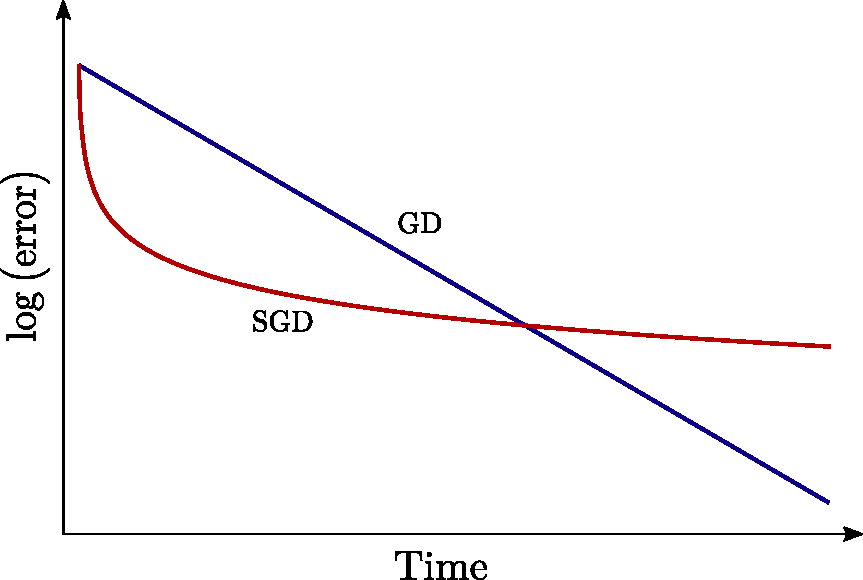
\includegraphics[width=0.6\textwidth]{figures/gd_sgd.pdf}
	\end{center}
\end{figure}

We see on the figure above that SGD obtains a decent solution reasonably fast. However, if one needs an high-accuracy solution, then standard gradient descent is more suitable.

In machine learning, objective functions are usually noisy because they depend on (noisy) data. That is, $R_N$ is equal to the true risk $R$, plus some errors.
Hence, there is no need to optimize $R_N$ with an accuracy below the noise level, which makes SGD particularly suitable for large-scale machine learning problems.



\section*{Further reading}

See chapter 9 of \cite{boyd2004convex} for more background on gradient descent and Newton's method.
See \cite{bottou2008tradeoffs} for a more in-depth analysis of the tradeoffs discussed in Section \ref{sec:concluding}.
See chapter 8 of \cite{goodfellow2016deep} for a discussion on the optimization of large neural nets.

\vspace{1cm}
\centerline{\pgfornament[width=7cm]{71}}


\bibliographystyle{plain}
\bibliography{../references.bib}

\section*{Appendix: Analysis of SGD for strongly convex objective functions}

In this section we assume $N$ to be very large, and typically larger than the total number of steps of SGD that we are going to make. This allows us to never use at each time $t$ a different gradient $\nabla f_{i_t}(\theta_t)$.


We start by rewriting SGD can be rewritten as
\begin{equation}\label{eq:sgd_noise}
\theta_{t+1} = \theta_t - \alpha_t \big(\nabla R(\theta_t) + \eps_t \big)
\end{equation}
where $\eps_t \defeq \nabla f_{i_t}(\theta_t) - \nabla R(\theta_t)$. 
We use this notation to make clear that $\nabla f_{i_t}(\theta_t)$ is a noisy observation of $\nabla R(\theta_t)$, where $\eps_t$ denotes the error.
Notice that $\E\big[\nabla f_{i_t}(\theta_t)| \theta_t\big] = \nabla R(\theta_t)$, thus $\E[\eps_t|\theta_t] = 0$.
We make the following additional assumptions:
\begin{itemize}
	\item There exists $\sigma>0$ such that $\E\big[\|\eps_t\|^2\big|\theta_t\big] \leq \sigma^2$ for all $t \geq 0$.
	\item $R$ is $\mu$-strongly convex and $L$-smooth.
	\item $\min_{\theta \in \R^n} R(\theta) =0$. (This can be easily verified by shifting $R$ by a constant.)
\end{itemize}
\vspace{2mm}
Applying $R$ on both sides of \eqref{eq:sgd_noise} and using the $L$-smoothness of $L$, we get
\begin{align*}
	R(\theta_{t+1}) \leq R(\theta_t) - \alpha_t \big\langle \nabla R(\theta_t), \nabla R(\theta_t) + \eps_t \big\rangle + \frac{L}{2} \alpha_t \| \nabla R(\theta_t) + \eps_t \|^2.
\end{align*}
Taking expectations on both sides gives:
\begin{align*}
\E R(\theta_{t+1}) 
&\leq \E R(\theta_t) - \alpha_t \E \big\| \nabla R(\theta_t)\big\|^2 + \frac{L}{2}\alpha_t^2 \left( \E \| \nabla R(\theta_t) \|^2 + \sigma^2 \right).
\\
&\leq \E R(\theta_t) - \frac{\alpha_t}{2} \E \big\| \nabla R(\theta_t)\big\|^2 + \frac{L}{2}\alpha_t^2 \sigma^2,
\end{align*}
assuming $\alpha_t \leq 1/L$.
By strong convexity we have (as in \eqref{eq:boundG}): $R(\theta) \leq 2 \mu \|\nabla R(\theta)\|^2$. Hence:
$$
\E R(\theta_{t+1}) \leq \left(1 - \mu \alpha_t\right)\E R(\theta_t)  + \frac{L}{2}\alpha_t^2  \sigma^2 .
$$
Using this inequalities, assuming that $(\alpha_t)_{t \geq 0}$ is non-increasing and less that $1/L$, one can prove that for all $0 \leq t \leq T$:
$$
\E [R(\theta_{T})] \leq \E \big[R(\theta_0)\big] \prod_{t=1}^T (1-\mu \alpha_t) 
+ \frac{L \sigma^2}{2} \exp\Big(-\mu \sum_{s=t+1}^T \alpha_t\Big) \sum_{t=1}^T \alpha_t^2 + \frac{L\sigma^2\alpha_t}{2\mu}.
$$

\paragraph{Analysis of the first term.}
When $\alpha_t \to 0$, 
$$\log \prod_{t=1}^T (1-\mu \alpha_t) =\sum_{t=1}^T \log (1-\mu \alpha_t) \sim - \mu \sum_{t=0}^{T} \alpha_t.$$
Hence, we need that $\sum_{t \geq 0} \alpha_t = +\infty$ in order to make the first term go to zero.
\\

\paragraph{Conclusion.}
Taking $\alpha_t = 1/(\mu t)$, we get:
$$
\E[R(\theta_T)] = O(1/T).
$$


\end{document}
